\documentclass[12pt,a4paper]{article}
\usepackage{comment}
\usepackage[hidelinks]{hyperref}
\usepackage{listings}
\usepackage{graphicx}
\graphicspath{{../Data_modelling/Assets}}

\usepackage{subcaption}
\usepackage{float}
\usepackage[table,xcdraw]{xcolor}
\usepackage{wrapfig}
\usepackage{tcolorbox}

\usepackage{xcolor}

\definecolor{codegreen}{rgb}{0,0.6,0}
\definecolor{codegray}{rgb}{0.5,0.5,0.5}
\definecolor{codepurple}{rgb}{0.58,0,0.82}
\definecolor{backcolour}{rgb}{0.95,0.95,0.92}

\lstdefinestyle{mystyle}{
    backgroundcolor=\color{backcolour},   
    commentstyle=\color{codegreen},
    keywordstyle=\color{magenta},
    numberstyle=\tiny\color{codegray},
    stringstyle=\color{codepurple},
    basicstyle=\ttfamily\footnotesize,
    breakatwhitespace=false,         
    breaklines=true,                 
    captionpos=b,                    
    keepspaces=true,                 
    numbers=left,                    
    numbersep=5pt,                  
    showspaces=false,                
    showstringspaces=false,
    showtabs=false,                  
    tabsize=2
}

\lstset{style=mystyle}

\title{%
    \vspace*{-5mm}\Huge \textbf{GW2-SRS} \\
    \vspace*{2mm}\Large powered by \LaTeX}

\author{\vspace*{-5mm}\large Daniel Lopez: \textbf{Project Documentation}}

\begin{document}
    \maketitle

    \begin{figure}[H]
        \centering
        
\includegraphics[width=1 \textwidth]{Images/Nuevo_logo_GW2.png}
    \end{figure}

    \newpage

    \begin{tcolorbox}
        I wanted to briefly explain why I started this project, since it is also important to
        know why people do what they do. I started SRS when I started my first Big Data course, I
        was quite fascinated since I've been always engaged with data, what it says of us and how
        the world is actually going towards use of data more and more to make choices. GW2-SRS is
        not only a project build to train Data Engineering techniques but also a tribute to one of 
        my favorite MMOs and the people I met playing it.\\

        \textbf{GW2-System for Raid Study} is my approach to analyze game data in Raids and make
        decisions based on what players do, play and how they perform overall.
    \end{tcolorbox}

    \section*{1.0 EXTRACT}

    \section*{\large 1.1 Introduction}
    As the first part of the \textbf{ETL} it's important to have in mind our data sources. When
    I began with the project I only had one way of getting logs, and they were all coming
    from friends. This meant I had to manually parse them with EliteInsights\footnote{EliteInsights it's an app designed to parse \textit{.zevtc} files into JSON, HTML or CSV files.}. 

    This process was extremely slow, and when at first it was viable due to having few logs,
    it started being quite useless when the project meant to have lots of logs to analyze.
    The best option then was thinking on using web-scraping or an API connection; and thankfully
    we have a web-page available, thanks to \textit{Johannes Pfau}, where people can upload their logs.\\

    \noindent \href{https://gw2wingman.nevermindcreations.de/home}{GW2-Wingman} is probably the best approach I made to this project, not only in efficiency, but also
    in learn curve. Scraping was something I craved for since I started focusing on the Data Engineering
    route. It taught me a lot of things and problems I could solve, some easier, some harder, but
    all of them were at the end solved.

    \newpage

    \section*{\large 1.2 About GW2-Wingman architecture}
    As I was learning to scrape the web-page I realized something wasn't right, and it made the scrape a
    bit harder when I understood the data was stored inside an \textbf{iframe tag}\footnote{An iframe is a nested web
    inside the main website}, so it was a matter of getting to the actual web-page.\\

    \noindent It was quite simple in the end, the iframe had an \textbf{href} tag containing the actual path, which only added
    \textit{/logContent} before the log name. \\

    \noindent This is a comparison of the actual URL showed, with the nested one:
    \begin{lstlisting}[language=Python]
    https://gw2wingman.nevermindcreations.de/log

    https://gw2wingman.nevermindcreations.de/logContent
    \end{lstlisting}

    \section*{\large 1.3 JSON data gathering}
    Extract algorithms are rather simple once you understand what you need to find, and that was
    the hardest part, since it required looking into the actual HTML code. I tackled the extraction
    with BeautifulSoup\footnote{As well as Selenium, BeautifulSoup let us extract information from any web-page.} 
    by passing an URL and the needed headers.\\

    \noindent After that I just needed to get the correct script and extract the JSON. This required a bit of 
    research; the JSON was nested on a JavaScript variable, which I had to strip off, and save only the
    JSON data.

    \begin{lstlisting}[language=Python]
    response = requests.get(url=url,headers=HEADERS)
    soup = BeautifulSoup(response.content,'html.parser')

    data = soup.find_all('script')[8]
    dataString = data.text.rstrip()
    \end{lstlisting}

    \newpage

    Last thing I needed to do is set up an algorithm, or in this case, a class, that help us know
    the boss Name and create a tag with it. This will make the further processes so much agile:

    \begin{lstlisting}[language=Python]
    class boss:

        def __init__(self, url: str) -> str:
            self.url = url

        def getBossName(self) -> str:
            url = self.url
            urlLines = url.split('/')
            if len(urlLines) < 5:
                bossName = urlLines[3]
            elif len(urlLines) == 5:
                bossName = urlLines[4]
            return bossName
        
        def getBossTag(self, bossName: str) -> str:
            bossTag = bossName.split('_')
            nameTag = bossTag[1]
            return nameTag
    \end{lstlisting}

    \section*{\large 1.4 URL copy code}
    Ending with the extraction part of the project, I will explain a quite relevant part here. 
    Normally we could extract information URL by URL, but it is not really convenient when we have, 
    like in this case, more than 100 logs. Therefore, best option is creating a script that copy and 
    write down this URLs for us on a text file we can later read.\\

    \begin{itemize}

        \item I set the search method to scope the 'a' tags, so I only had to just take the href of each one and 
        add the url\_str and have the complete link for a later iteration.

        \item Nonetheless, the 'a' tag contains about 5-6 lines that are not log hrefs, instead, they show an apikey 
        href and JavaScript void hrefs, so I just omitted them and set a new line for each one the script finds.

        \newpage

        \item Finally, I wrote it down on a .txt file; however I realized that, at first I was using 'w' mode, but it 
        ended being quite inefficient since it constantly overwrites the file. To avoid this, I just simply changed 
        the 'w' mode to 'a'\footnote{An 'a' stands for append, and will add new data without overwriting the existing one}
        mode, this way we can just append the information and not worry about it overwriting over and over again.

    \end{itemize}

    This is how the code looks like:

    \begin{lstlisting}[language=Python]
    fh = open(path,'a')

    for link in soup.find_all('a'):
        url_str = 'https://gw2wingman.nevermindcreations.de'
        data = link.get('href')
        
        try:
            log_str = url_str+data
            if log_str.endswith('apikey'):
                log_str.replace('apikey','\n')
            elif log_str.endswith('void(0)'):
                log_str.replace('void(0)','\n')
            else:
                fh.write(log_str)
                fh.write('\n')
        except Exception as e:
            print('Error: ', str(e))
    \end{lstlisting}

    \newpage

    \section*{2.0 TRANSFORM}

    \section*{\large 2.1 Introduction}
    After completing the data extraction, it was needed to do a deep cleaning on the files.
    The extracted data was displayed on the HTML source as a JSON type, it as well contained
    lots of information that is entirely related to the statistics in-game. Whether is true that
    statistics showed player names, player accounts, DPS\footnote{Damage Per Second}, etc. It
    also showed information that wasn't needed at all, where we could find EliteInsights information
    about it's version, release and EVTC\footnote{Unique log filetype from ArcDPS app} version as well.\\

    Therefore, I only wanted to gather clear stats data that could help me in the further
    analysis. The data I decided to aim for was:
    \begin{itemize}
        \item Player name
        \item Player Account
        \item Player Profession/Class
        \item Player DPS Statistics
    \end{itemize}

    \begin{table}[!h]
        \begin{tabular}{|c|llll}
        \hline
                                           & \multicolumn{1}{c|}{\cellcolor[HTML]{CBCEFB}Player's Name} & \multicolumn{1}{c|}{\cellcolor[HTML]{CBCEFB}Player's Account} & \multicolumn{1}{c|}{\cellcolor[HTML]{CBCEFB}Player's Class} & \multicolumn{1}{c|}{\cellcolor[HTML]{CBCEFB}Player's DPS} \\ \hline
        \cellcolor[HTML]{FFCCC9}\textbf{1} & \multicolumn{1}{c}{John\_Doe}                              & \multicolumn{1}{c}{johndoe.9752}                              & \multicolumn{1}{c}{Catalyst}                                & \multicolumn{1}{c}{35867.43}                              \\ \cline{1-1}
        \cellcolor[HTML]{FFCCC9}\textbf{2} & ...                                                        &                                                               &                                                             &                                                           \\ \cline{1-1}
        \cellcolor[HTML]{FFCCC9}\textbf{3} &                                                            &                                                               &                                                             &                                                           \\ \cline{1-1}
        \end{tabular}
    \end{table}

    \newpage

    \section*{\large 2.2 In-depth data explanation}

    \subsection*{\normalsize 2.2.1 JSON format}
    In order to understand the data, I had to read and investigate the JSON files lots of times.
    Due to the JSON files size, I decided to use a JSON Viewer\footnote{http://jsonviewer.stack.hu/} 
    to help me with this task.\\

    \begin{figure}[h!]
        \centering
        \begin{subfigure}[b]{0.8\linewidth}
          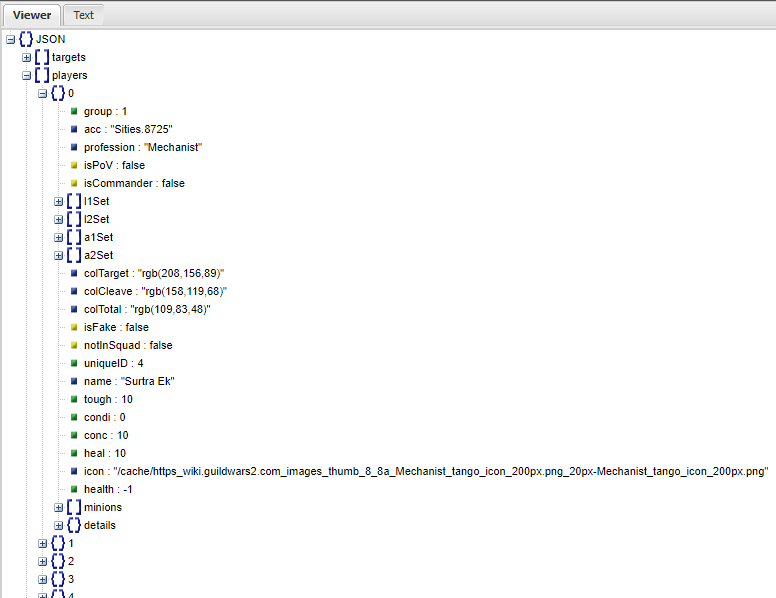
\includegraphics[width=\linewidth]{Images/json_schema.png}
          \caption{JSON Viewer formatted schema}
        \end{subfigure}

        \begin{subfigure}[b]{0.8\linewidth}
          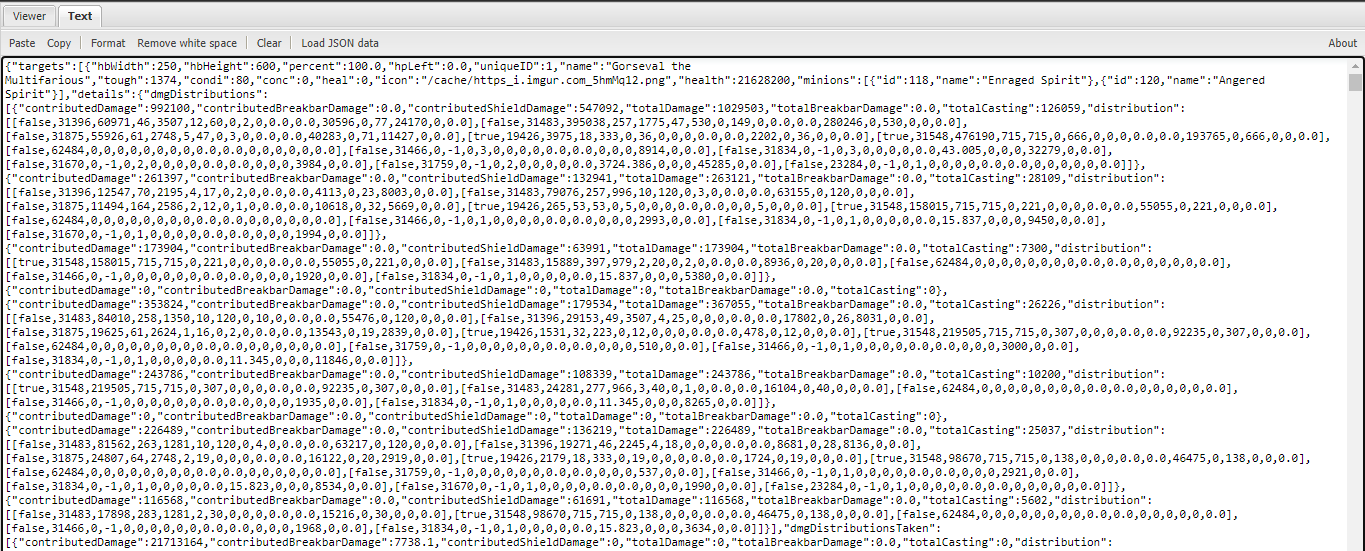
\includegraphics[width=\linewidth]{Images/json_raw.png}
          \caption{Raw JSON view}
        \end{subfigure}
    \end{figure}

    \newpage

    Using this method made the search of information extremely easy, for the most part, the essential
    player data like names, accounts and professions was pretty much finding each player and this data
    by it's index. I applied a zipped For loop to do the aggregation on SQL databases and on No-SQL databases
    I used a simple dictionary I created and then passed as a JSON dictionary.\\

    \begin{lstlisting}[language=Python, caption={\textbf{Basic player data loop}},captionpos=!b]
        for player in data['players']:
            player_group.append(player['group'])
            player_acc.append(player['acc'])
            player_names.append(player['name'])
            player_classes.append(player['profession'])
    \end{lstlisting}
    \begin{lstlisting}[language=Python, caption={\textbf{Custom Python stat dictionary}},captionpos=!b]
        stats_dict = {
                'boss': target,
                'players':{
                    'group': player_group,
                    'account': player_acc,
                    'names': player_names,
                    'profession': player_classes,
                    'phase_1_dps': player_dps1,
                    'phase_2_dps': player_dps2,
                    'phase_3_dps': player_dps3
                }
            }
    \end{lstlisting}
    
    \begin{lstlisting}[language=Python, caption={\textbf{Zipped data for SQLite query}},captionpos=!b]
        for (name,acc,profession) in zip \
        (player_names,player_acc,player_classes):
    \end{lstlisting}

    It was important using a zipped For loop since the query need to be executed for every player.
    This is indeed not efficient if we look into the repetition of the same query for a simple operation
    but since there are only 10 players per boss fight, it ended up being rather useful.

    \newpage

    \subsection*{\normalsize 2.2.2 DPS data}
    Finding each boss DPS data was indeed a quite difficult task. In order to get deeper in this topic
    I must explain a few concepts from Guild Wars 2 game itself.

    Guild Wars 2 is an MMO, and have different classes or profession that the player can create, however, in
    raid, strikes and fractals, we must have in mind that classes have two kind of damage: Condition damage
    and Power damage. This is important to understand since the DPS on each boss, and for each player, is divided
    between Condition and Power as well as it has a combination of both.

    Every class in the game can deal both Power and Condition, but some classes are more suitable to deal Power
    damage and some other classes are more suitable to deal Condition damage.

    Once explained this, we can get a bit deeper into the data. As I said before, the DPS data has three values
    per phase:
    \begin{itemize}
        \item Power + Condition
        \item Condition
        \item Power
    \end{itemize} 

    There is more data stored in the JSON, but what I needed is essentially this. I used the combined one, and
    you may wonder why not use the specific damage for each class. This not only could be extremely inefficient in
    the long run, but also, damage is also affected but extra aspects and boons added by other classes, so even if
    you are a Power class, you could get a buff from a Thief class making your attacks deal Poison damage which is 
    considered a Condition. Therefore, using the combined one is rather a better option.

    \newpage

    Another important fact to know is that, each boss has different phases. It's true that some bosses share same phases
    and same index, but this does not represent the majority of the bosses. Therefore, each boss needs its own index
    finder. It looks like this in the actual code:

    \begin{lstlisting}[language=Python]
    if nameTag == 'vg':

            # Phase_1
            phase1 = data['phases'][1]['dpsStats']

            phase1_time_raw = data['phases'][1]['duration']
            phase1_time = round(phase1_time_raw/1000,1)

            for dps in phase1:
                dps1_raw = dps[0]
                player_dps1.append(round(dps1_raw/phase1_time,2))

            # Phase_2
            phase2 = data['phases'][6]['dpsStats']

            phase2_time_raw = data['phases'][6]['duration']
            phase2_time = round(phase2_time_raw/1000,1)

            for dps in phase2:
                dps2_raw = dps[0]
                player_dps2.append(round(dps2_raw/phase2_time,2))

            # Phase_3
            phase3 = data['phases'][12]['dpsStats']

            phase3_time_raw = data['phases'][12]['duration']
            phase3_time = round(phase3_time_raw/1000,1)

            for dps in phase3:
                dps3_raw = dps[0]
                player_dps3.append(round(dps3_raw/phase3_time,2))
    \end{lstlisting}

    \newpage

    We are applying several things here. For instance, every boss has between 3 and 6 phases where you can actually damage it,
    this doesn't mean that there are no extra phases, but the damage there is really not that important or substantial to have
    it in mind for an analysis. Therefore, I picked the main phases and made a set of operations over it:

    \begin{itemize}
        \item I applied a For loop on every phase, so it saves the damage dealt for every player.
        \item This information is appended to an empty list.
        \item Finally, but really important, all the damage is divided by the time phase.
    \end{itemize}

    \bigskip

    If we look at the JSON file, it's easy to see that all phase timestamps are written like a single int number (i.e: 190s = 190000),
    this was actually problematic when trying to divide the phase dmg numbers. So the best option I found to deal with this problem
    was dividing it by 1000 so it shows time in seconds and therefore division could be executed better. To end with this data, I just
    applied a \textbf{round} operation.

    \newpage

    \section*{3.0 LOAD}

    \section*{\large 3.1 Introduction}
    The last part concerning the ETL process is loading the results into a database. 
    In this case I decided going for MongoDB and SQLite.
    The reason behind this decision was storing big JSON files in a suitable database like MongoDB, while
    maintaining an space for structured tables on SQLite that I built with queries.\\

    Now the key part here, is that at first I was saving entire JSONs on MongoDB, and while this is the
    purpose of a No-SQL database, I preferred just uploading the dictionaries I created manually within the
    ETL code. As for SQLite, there are two main queries, one for dps data and one for users.

    \section*{\large 3.2 SQLite Queries}
    In order to have every boss classified, I created a table for each boss, so the data loading was a matter
    of inserting the data within the ETL, therefore I needed a connection with the database.\\

    I used Python and sqlite3\footnote{sqlite3 is a Python library used to work with SQLite database} to set 
    up the connection and execute the queries. The main connection can be set up using the following:

    \begin{lstlisting}[language=Python, caption=SQLite Connection]
        conn = sqlite3.connect("Your_database_path")
        cur = conn.cursor()
    \end{lstlisting}

    \bigskip

    From this line, we can easily execute any query inside the database by calling the cursor:

    \begin{lstlisting}[language=Python, caption=Query example]
        cur.execute(
            f"INSERT INTO vg_dps(phase1_dps,phase2_dps,phase3_dps,FK_player_id) \
            VALUES({dps1},{dps2},{dps3},'{acc}')"
        )
    \end{lstlisting}

    \newpage

    \section*{3.3 MongoDB Connection}
    As for MongoDB, the connection is quite simple as well. I chose to use PyMongo library and 
    a MongoDB Atlas Cluster to help me out. I used the local cluster, but this process could also
    be made on the cloud cluster as well. The connection would look like the following:

    \begin{lstlisting}[language=Python, caption=MongoDB Connection]
        client = pymongo.MongoClient('mongodb://localhost:27017/')
    \end{lstlisting}

    \begin{lstlisting}[language=Python, caption=MongoDB data load]
        db = client['GW2_SRS']
        collection = db['players_info']

        collection.insert_one(json_data)
        print('MongoDB load done!')
    \end{lstlisting}

    \newpage

    \section*{4.0 DATA MODELLING}

    \section*{\large 4.1 Introduction}
    \subsection*{\normalsize 4.1.1 Dates and Data}
    All the data used in this study is based on the class performance between May and September. This means
    that, with future nerfs and buffs to classes, values can easily vary. Therefore, this information is only
    relevant in those months. Nonetheless, some classes does not change a lot, so not every value has a chance
    to change.\\

    \subsection*{\normalsize 4.1.2 Model explanation}
    This project data was easier to store on MongoDB than it was on SQL, therefore, a data model was needed not
    only to connect data between tables, but also to have a data schema and keep everything ordered.

    The basic structure of data on MongoDB was explained on the previous EXTRACT part, as the info was saves with
    that specific schema. In SQLite, I needed to create several tables:

    \begin{itemize}
        \item Player's info
        \item Boss names
        \item Profession names
        \item DPS Tables for each boss
    \end{itemize}
    
    \bigskip

    The first table in the list contains names, accounts and two more columns, one of the columns contains a Foreign
    Key (\textbf{FK}) that connects to Boss Names by its Primary Key (\textbf{PK}), as for the second one, it
    contains another FK that connects to Profession names PK. Boss Names and Profession Names are two tables that
    only contains a PK and the names respectively. This was designed this way to prevent data repeating over and over
    when using a PK and FK was by far, the best option.

    \newpage

    Inside the DPS Tables, I had quite a few problems linking data between tables. The DPS tables stored data based 
    on an ID as well, but if \textit{JohnDoe.9100} had ID 30 on the players table and his damage in Vale Guardian corresponds 
    to ID 2 it wouldn't work at all, there was no connection and therefore it leads to error.\\

    The solution was not what I would have done if I had other options in mind, however, it worked fine. I created a FK 
    for every dps table that contained the user account, this way we could just refer the FK to the players table and get 
    the connection done. I thought on doing it with the boss number, but it could also resulted in some problems.

    This choice was mainly done because we use ID as a unique value that represents something, and actually, in a game, your 
    account name is already a unique value that identifies the player and it's also \textbf{immutable}.

    \section*{\large 4.2 Results, Graphs and Analysis}
    The analysis on the project has two main objectives:

    \begin{itemize}
        \item Profession/Class Usage per boss
        \item DPS done per class on each boss
    \end{itemize}

    \bigskip

    \subsection*{\normalsize 4.2.1 Profession/Class Usage}

    \begin{figure}[h!]

        \centering

        \begin{subfigure}{0.5\textwidth}
            \centering
            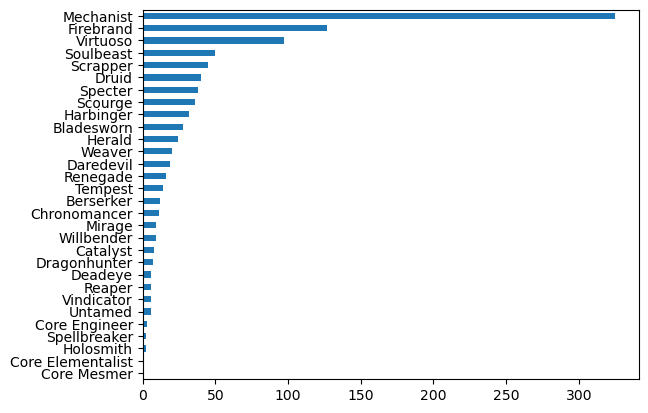
\includegraphics[scale=0.4]{vg_graph.png}
            \caption{\small W1: Vale Guardian Graph}
        \end{subfigure}%
        \begin{subfigure}{0.5\textwidth}
            \centering
            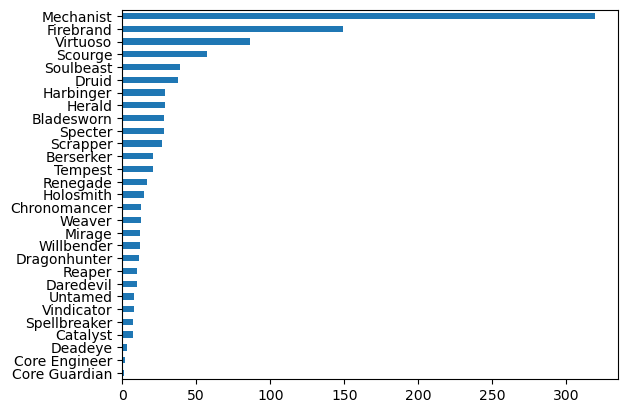
\includegraphics[scale=0.4]{gors_graph.png}
            \caption{\small W1: Gorseval Graph}
        \end{subfigure}
    \end{figure}

    \newpage

    \begin{figure}[h!]

        \centering

        \begin{subfigure}{0.5\textwidth}
            \centering
            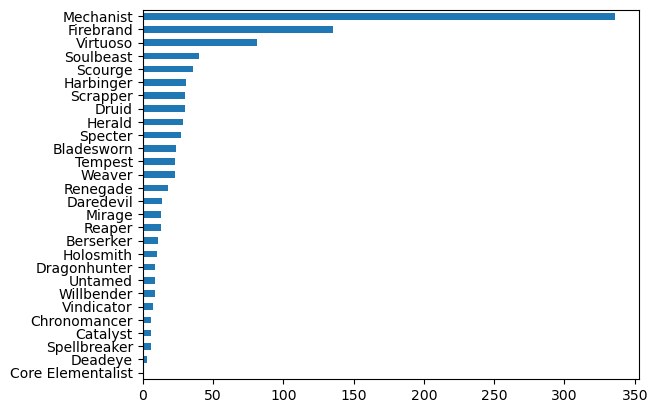
\includegraphics[scale=0.4]{sab_graph.png}
            \caption{\small W1: Sabetha Graph}
        \end{subfigure}%
        \begin{subfigure}{0.5\textwidth}
            \centering
            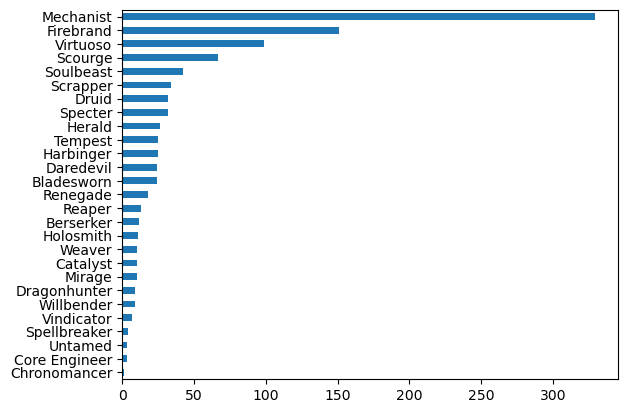
\includegraphics[scale=0.4]{sloth_graph.png}
            \caption{\small W2: Slothasor Graph}
        \end{subfigure}

        \begin{subfigure}{0.5\textwidth}
            \centering
            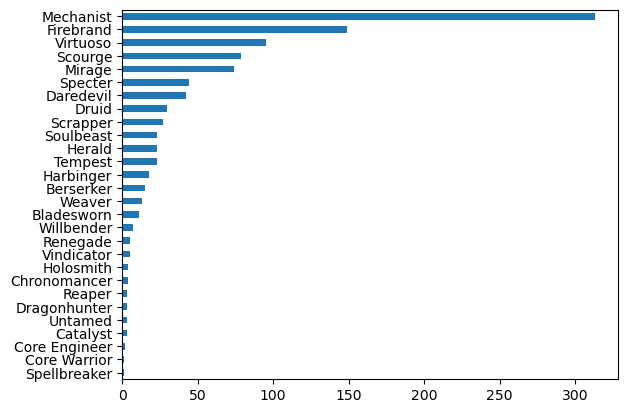
\includegraphics[scale=0.4]{matt_graph.png}
            \caption{\small W2: Matthias Gabrel Graph}
        \end{subfigure}%
        \begin{subfigure}{0.5\textwidth}
            \centering
            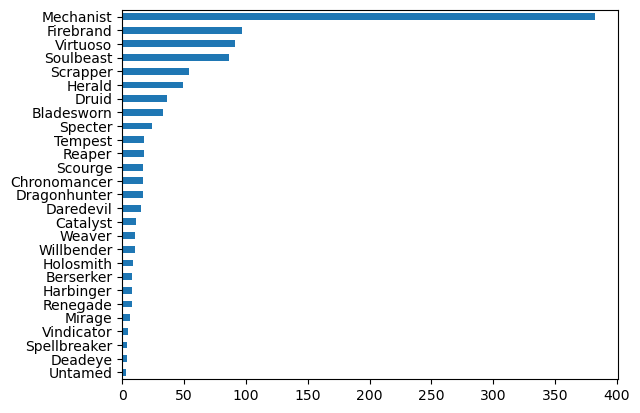
\includegraphics[scale=0.4]{kc_graph.png}
            \caption{\small W3: Keep Construct Graph}
        \end{subfigure}

        \begin{subfigure}{0.5\textwidth}
            \centering
            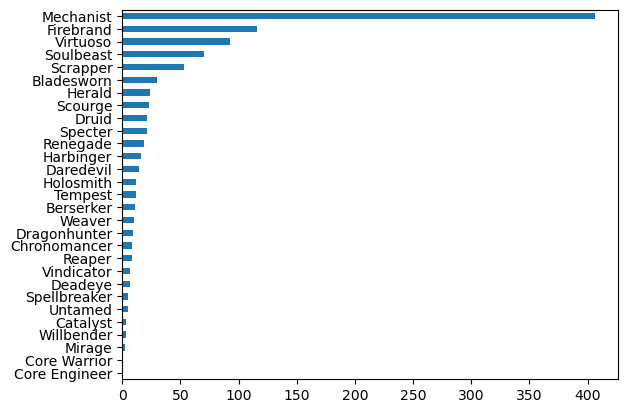
\includegraphics[scale=0.4]{xera_graph.png}
            \caption{\small W3: Xera Graph}
        \end{subfigure}%
        \begin{subfigure}{0.5\textwidth}
            \centering
            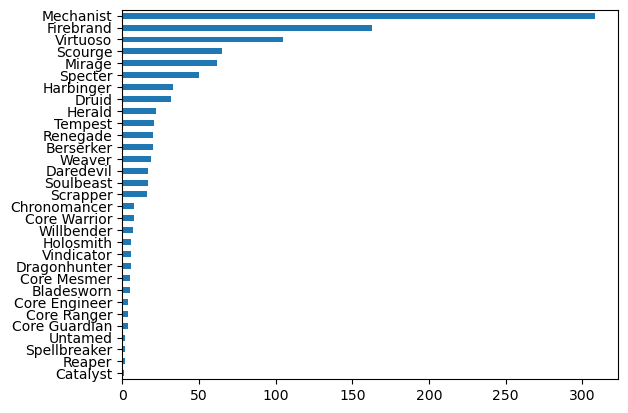
\includegraphics[scale=0.4]{cairn_graph.png}
            \caption{\small W4: Cairn Graph}
        \end{subfigure}

        \begin{subfigure}{0.5\textwidth}
            \centering
            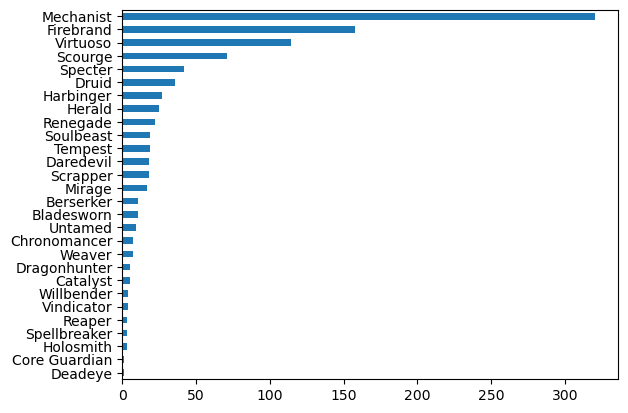
\includegraphics[scale=0.4]{mo_graph.png}
            \caption{\small W4: Mursaat Graph}
        \end{subfigure}%
        \begin{subfigure}{0.5\textwidth}
            \centering
            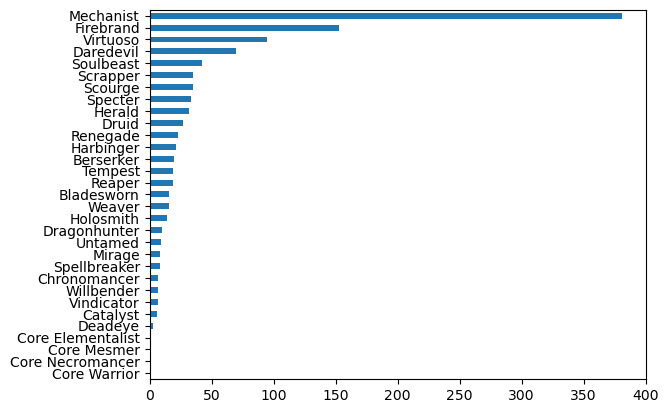
\includegraphics[scale=0.4]{sam_graph.png}
            \caption{\small W4: Samarog Graph}
        \end{subfigure}
    \end{figure}

    \newpage

    \begin{figure}[h!]
        
        \centering

        \begin{subfigure}{0.5\textwidth}
            \centering
            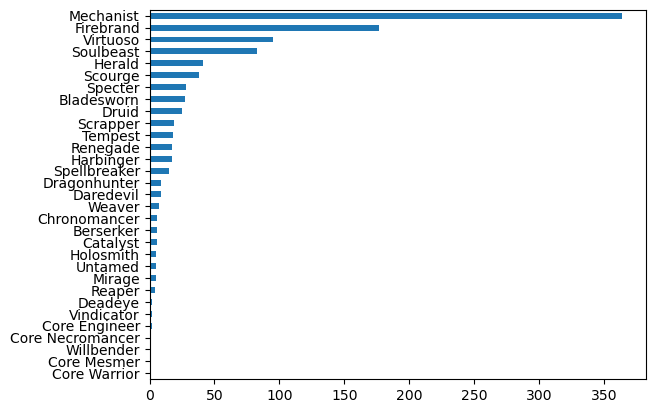
\includegraphics[scale=0.4]{dei_graph.png}
            \caption{\small W4: Deimos Graph}
        \end{subfigure}%
        \begin{subfigure}{0.5\textwidth}
            \centering
            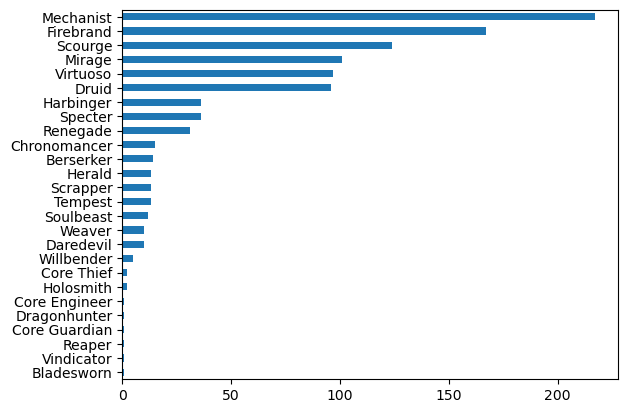
\includegraphics[scale=0.4]{sh_graph.png}
            \caption{\small W5: Soulless Horror Graph}
        \end{subfigure}

        \begin{subfigure}{0.5\textwidth}
            \centering
            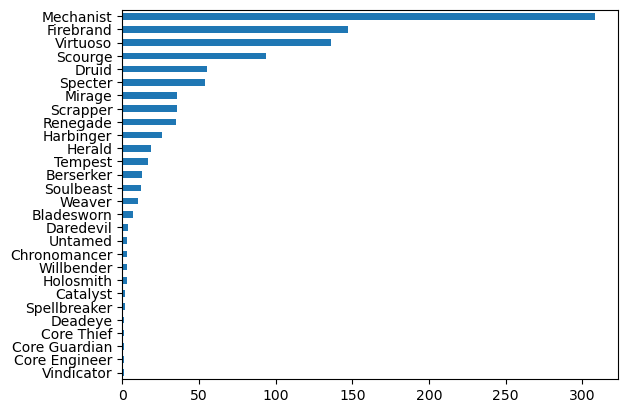
\includegraphics[scale=0.4]{dhuum_graph.png}
            \caption{\small W5: Dhuum Graph}
        \end{subfigure}%
        \begin{subfigure}{0.5\textwidth}
            \centering
            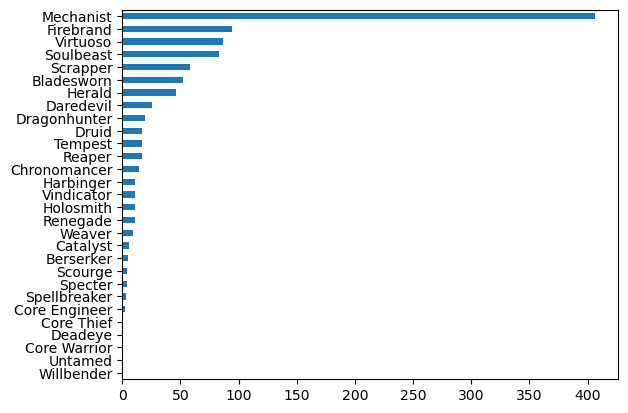
\includegraphics[scale=0.4]{ca_graph.png}
            \caption{\small W6: Conjured Amalgamate Graph}
        \end{subfigure}

        \begin{subfigure}{0.5\textwidth}
            \centering
            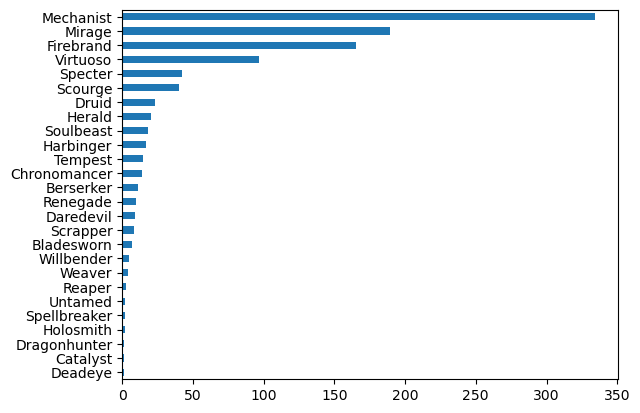
\includegraphics[scale=0.4]{twins_graph.png}
            \caption{\small W6: Twin Largos Graph}
        \end{subfigure}%
        \begin{subfigure}{0.5\textwidth}
            \centering
            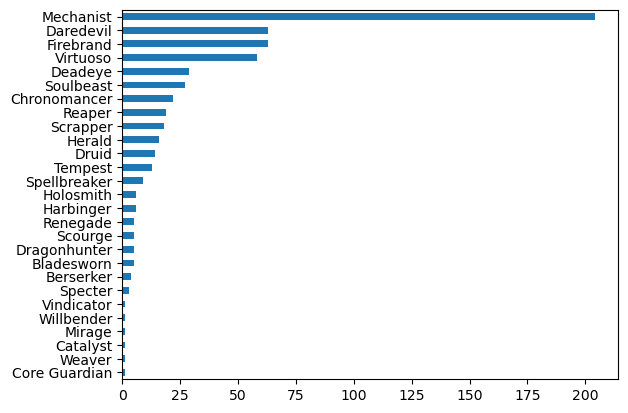
\includegraphics[scale=0.4]{q1_graph.png}
            \caption{\small W6: Qadim Graph}
        \end{subfigure}

        \begin{subfigure}{0.5\textwidth}
            \centering
            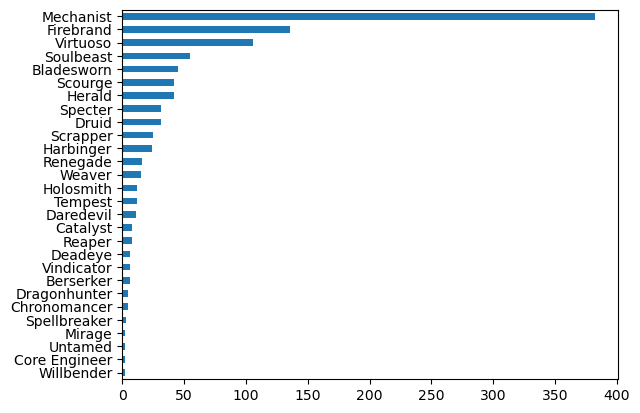
\includegraphics[scale=0.4]{adina_graph.png}
            \caption{\small W7: Cardinal Adina Graph}
        \end{subfigure}%
        \begin{subfigure}{0.5\textwidth}
            \centering
            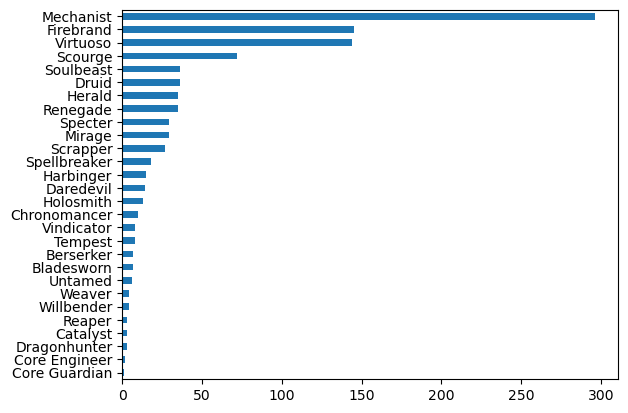
\includegraphics[scale=0.4]{sabir_graph.png}
            \caption{\small W7: Cardinal Sabir Graph}
        \end{subfigure}
    \end{figure}

    \newpage

    \begin{wrapfigure}{r}{0.5\textwidth}
        \centering
        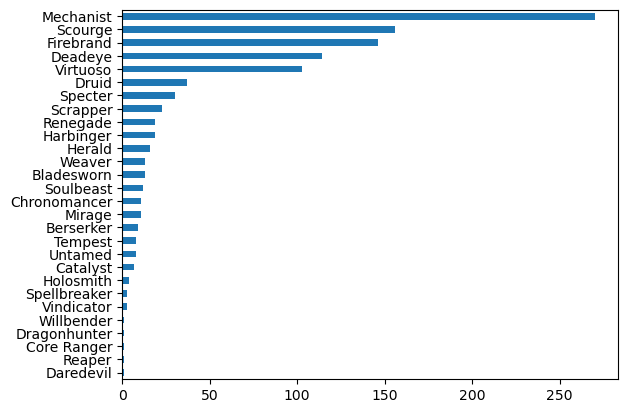
\includegraphics[scale=0.4]{prlqadim_graph.png}
        \caption{\small W7: Peerless Qadim Graph}
    \end{wrapfigure}

    All this graphs represent the class usage in each boss, and it stands out that the usage of
    the Mechanist class is huge. Just to be clear, \textbf{all this analysis is made from data 
    between May and September 2022}, therefore, during this period, Mechanist was a rather new 
    class since Guild Wars 2: End of Dragons came out in February 2022.\\

    Since the release of the Mechanist, as well as other classes, it became one of the best choices
    because it could be either support or dps, and it's results in raid were extremely good. We can 
    also see that other classes such as Firebrand is also quite high on the graph, and this is also
    due to Firebrand's versatility. Guild Wars 2 is a game where versatility in terms of raid and 
    fractals is really important, abilities that can provide \textbf{aegis}, \textbf{alacrity} and 
    \textbf{quickness} are three of the key support buffs, while \textbf{power} and \textbf{fury}
    are two of the key damage buffs. This is why classes like Guardian and Engineer are always on 
    top of the usage graphs.\\

    Each boss also has certain classes that perform better than others, as some bosses are weaker to
    condition damage and other bosses to power damage. On top of that, each boss also has certain
    mechanics, which normally needs certain classes to perform those specific roles; as an example,
    Peerless Qadim has the \textbf{Pylon} mechanic, and it's normally performed by Deadeyes or Scourges.

    \subsection*{\normalsize 4.2.2 DPS Data Graphs}
    Now that class usage have been seen, it's time to focus a little on dps data. This time, as earlier,
    I did a series of graphs that represent the damage done per class in each boss and on each phase. DPS
    stats seen in graphs are a mean of all the 1000+ rows on each boss table.

    \newpage

    \begin{figure}[h!]
        
        \centering
        
        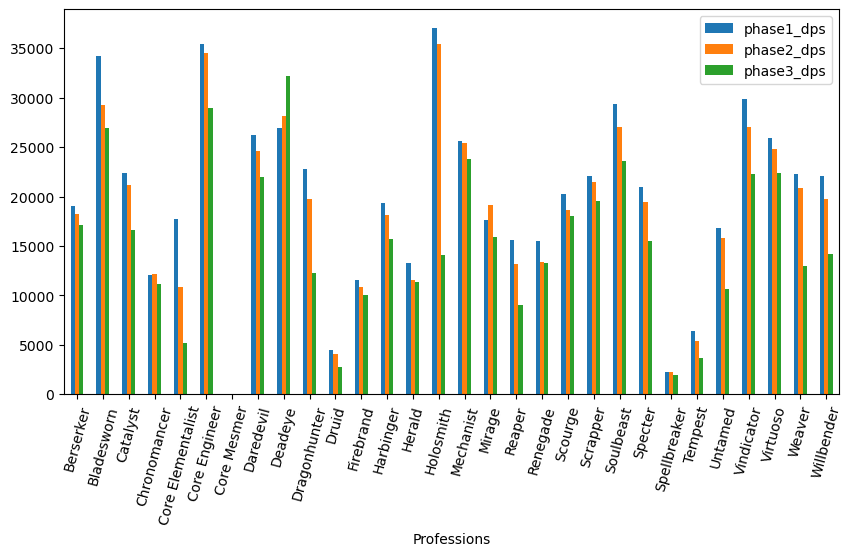
\includegraphics[width=1 \linewidth]{vg_dps_plot.png}
        \caption{Vale Guardian}
        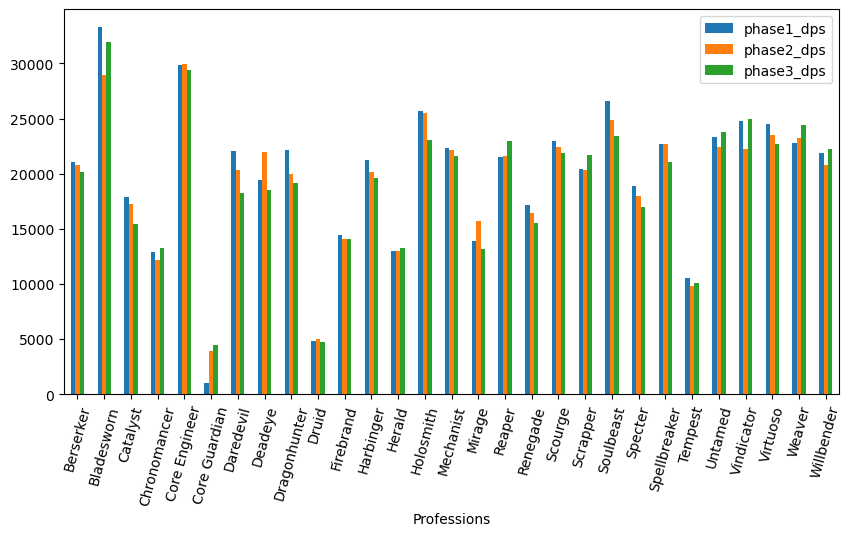
\includegraphics[width=1 \linewidth]{gors_dps_plot.png}
        \caption{Gorseval The Multifarious}
    \end{figure}

    \newpage

    \begin{figure}[h!]
        
        \centering
        
        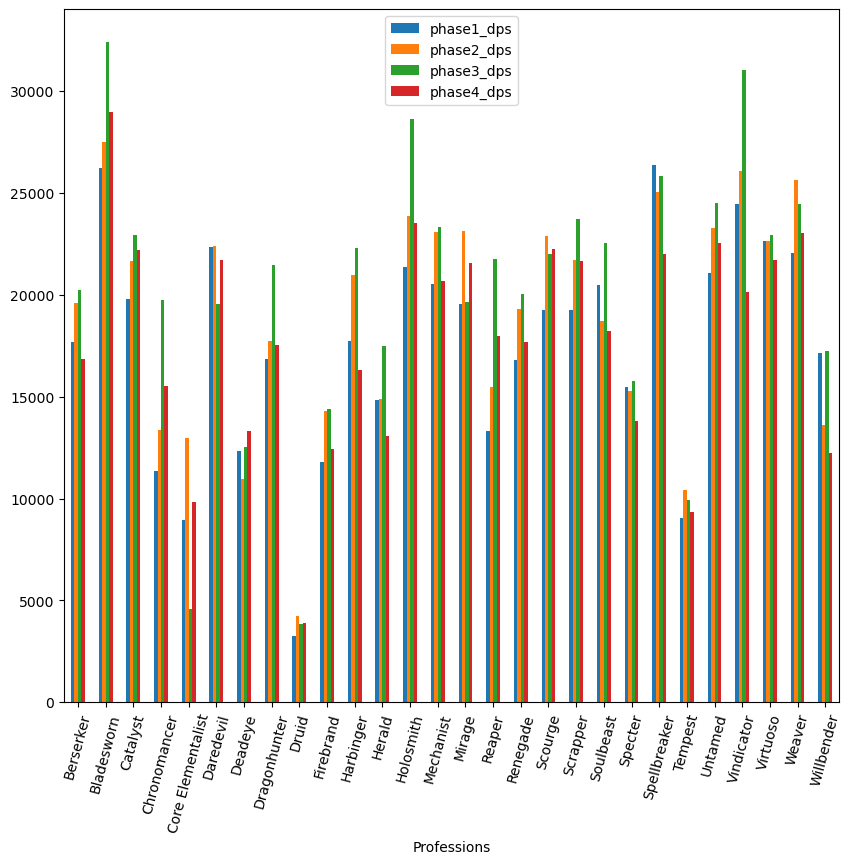
\includegraphics[width=1 \linewidth]{sab_dps_plot.png}
        \caption{Sabetha The Saboteur}
    \end{figure}

    Some plots had to be adjusted due to bosses having too many phases, normally bosses have few phases,
    however, I had to adapt the phase system EliteInsights have, which is mainly obtained from the game
    itself.\\

    In Sabetha's battle, there is a main mechanic consisting on destroying cannons that continuously attack
    the battle platform. If the platform falls due to damage, it will destroy and the battle will be lost.
    Therefore, two players are focused on destroying those cannons in an specific timing, while the rest of
    the team fights Sabetha and her minions.

    \newpage

    \begin{figure}[h!]
        
        \centering
        
        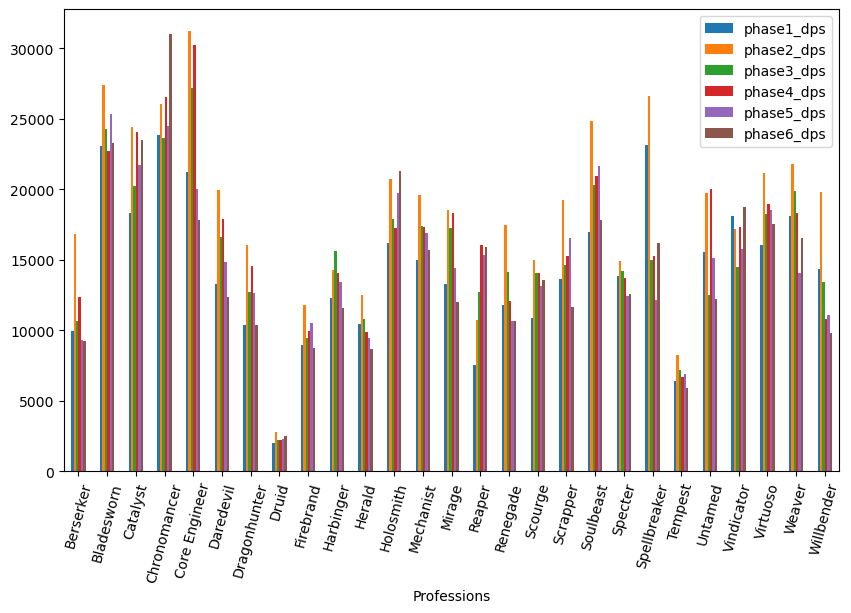
\includegraphics[width=1 \linewidth]{sloth_dps_plot.png}
        \caption{Slothasor}
    \end{figure}

    Slothasor is a boss with many phases due to his main mushroom mechanic. It consists of four mushrooms
    that need to be picked in order to clean areas and avoid stepping into venomous floor that kills the
    player slowly. When you pick this mushrooms, your character will stop doing damage to the boss and it
    will turn an enemy target for anyone on your team, therefore, players must be careful not to kill the
    teammate doing this mechanic.\\

    Added to this mechanic, Slothasor will shake his body from time to time causing several conditions on
    players that must be cleaned. Slothasor will also smash the ground and create three blue areas that 
    players need to dodge or else, they will be stunned for a while.\\

    Last mechanic is an active ability that will appear on a random player, this ability is a poison that 
    will drain player's life until he release the ability, and this must be done out of the group as it 
    creates a venomous pool that will also damage other teammates.

    \newpage

    \begin{figure}[h!]
        
        \centering
        
        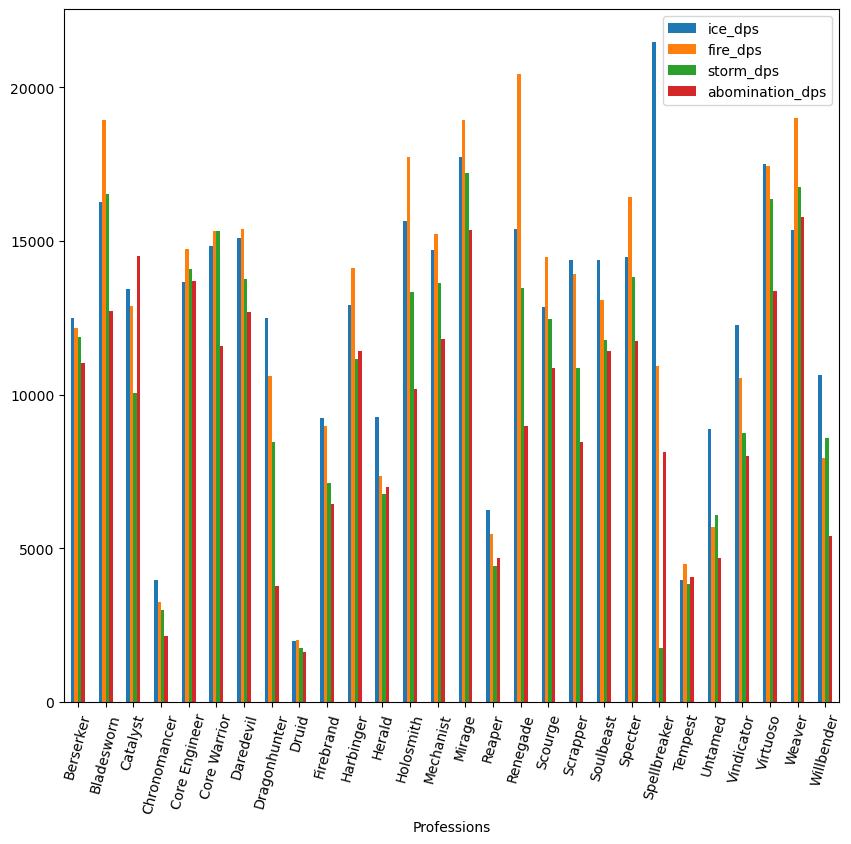
\includegraphics[width=1 \linewidth]{matt_dps_plot.png}
        \caption{Matthias Gabrel}
    \end{figure}

    Matthias battle is quite special, as its phases are based on a weather happening on the battlefield and
    it affects players as well: ice will slow players, fire will create tornados damaging and stunning players...
    The abomination phase is the one that combines every effect happening before plus, Matthias becomes a bigger
    creature that will have the same movements as the original Matthias.

    \newpage

    \begin{figure}[h!]
        
        \centering
        
        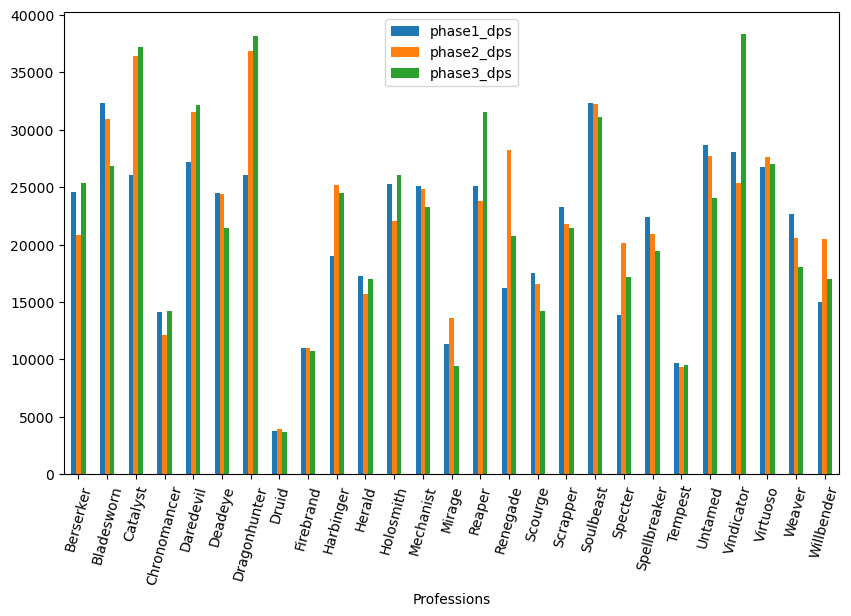
\includegraphics[width=1 \linewidth]{kc_dps_plot.png}
        \caption{Keep Construct}
        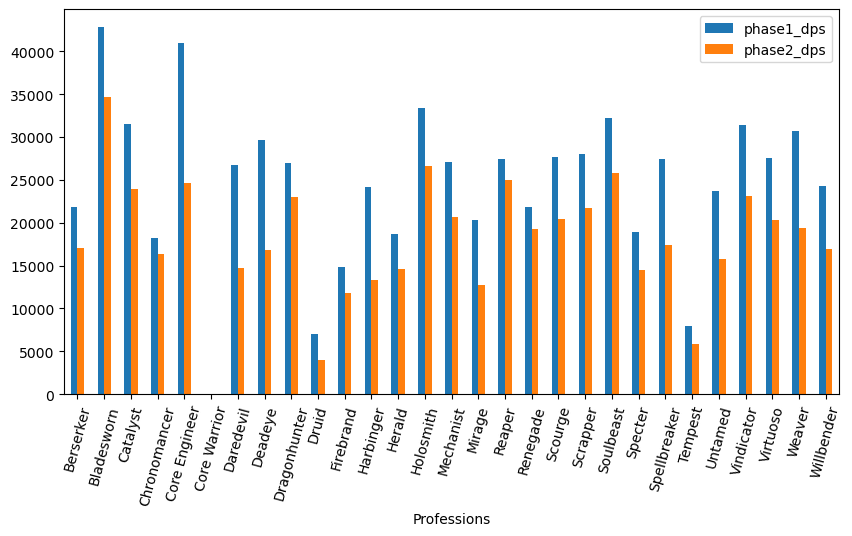
\includegraphics[width=1 \linewidth]{xera_dps_plot.png}
        \caption{Xera}
    \end{figure}

    \newpage

    \begin{figure}[h!]
        
        \centering
        
        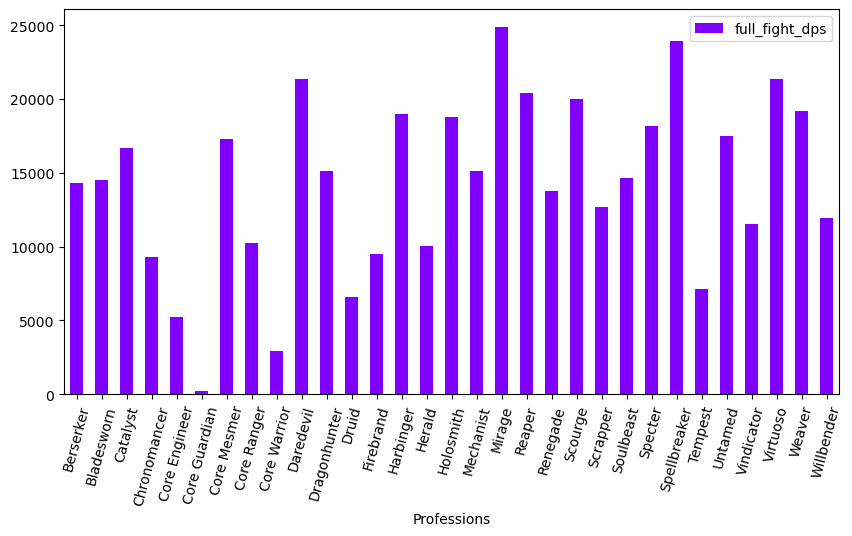
\includegraphics[width=1 \linewidth]{cairn_dps_plot.png}
        \caption{Cairn The Indomitable}
        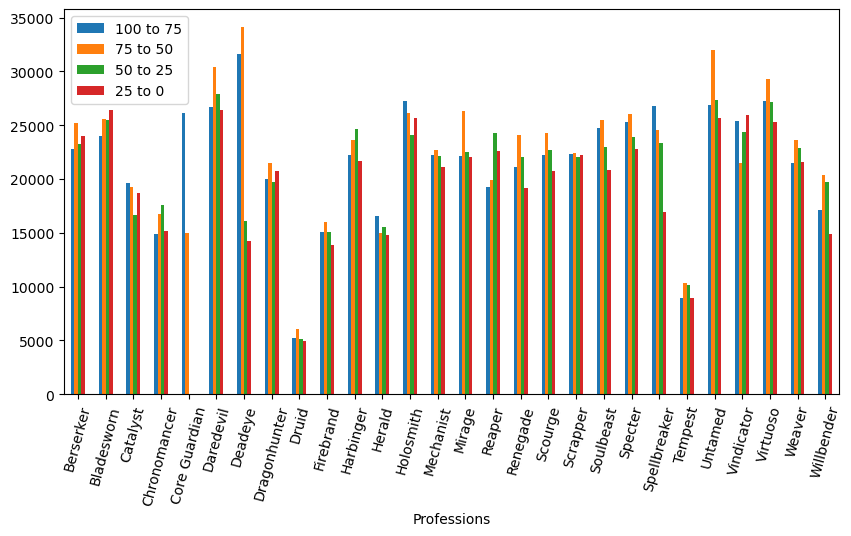
\includegraphics[width=1 \linewidth]{mo_dps_plot.png}
        \caption{Mursaat Overseer}
    \end{figure}

    \newpage

    \begin{figure}[h!]
        
        \centering
        
        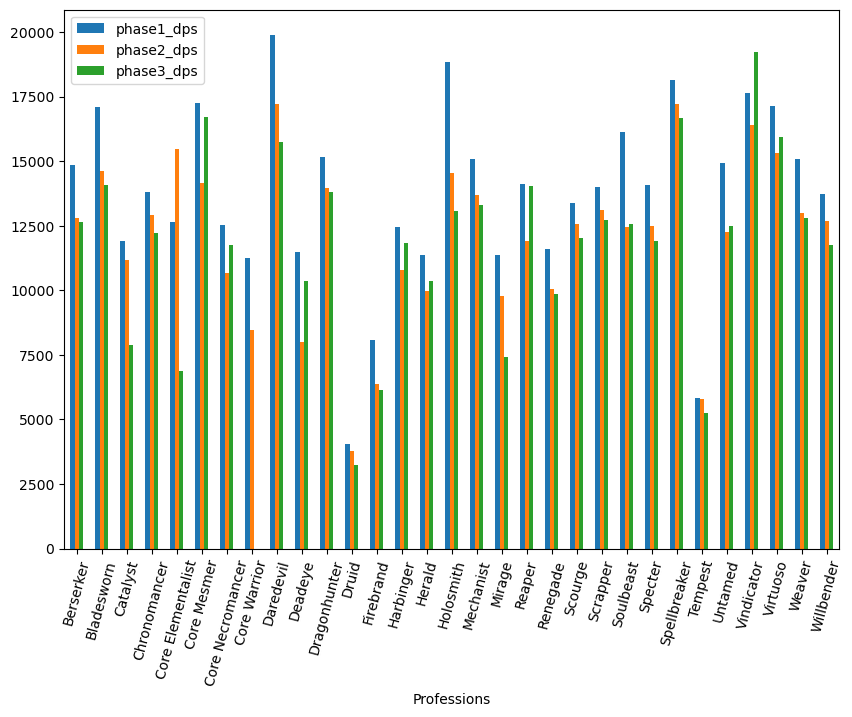
\includegraphics[width=1 \linewidth]{sam_dps_plot.png}
        \caption{Samarog}
    \end{figure}

    As seen before, there are also bosses like Cairn that have a single phase, and this is due the kind of battle
    it has. Cairn battle it's based on a 100 to 0 battle, it has certain mechanics that everyone needs to do, but
    those mechanics doesn't stop some players from doing damage or being outside of the group needing to have in 
    certain objectives in mind. A way to explain this would be Samarog; his battle is quite straight-forward, but,
    at every 33\% HP lost he will exit the battlefield and another fight phase with two other enemies will began.

    \newpage

    \begin{figure}[h!]
        
        \centering
        
        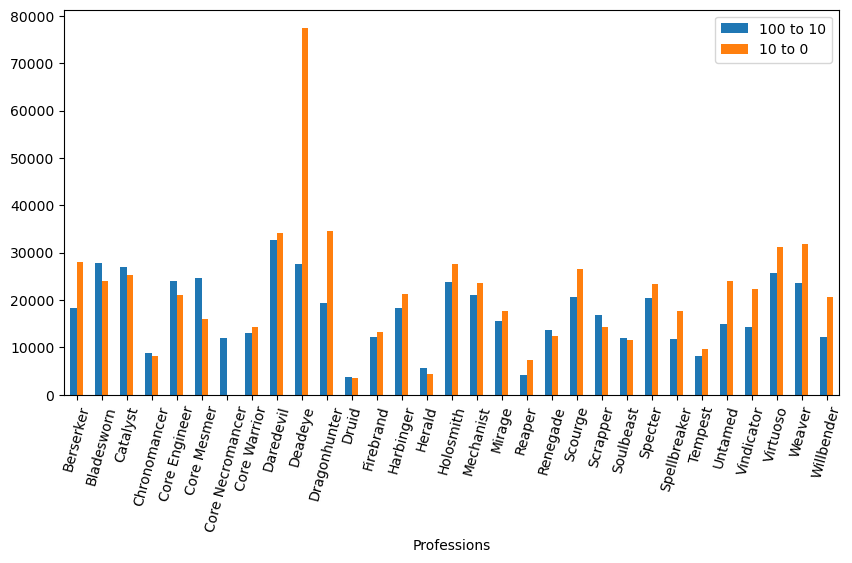
\includegraphics[width=0.8 \linewidth]{dei_dps_plot.png}
        \caption{Deimos}
        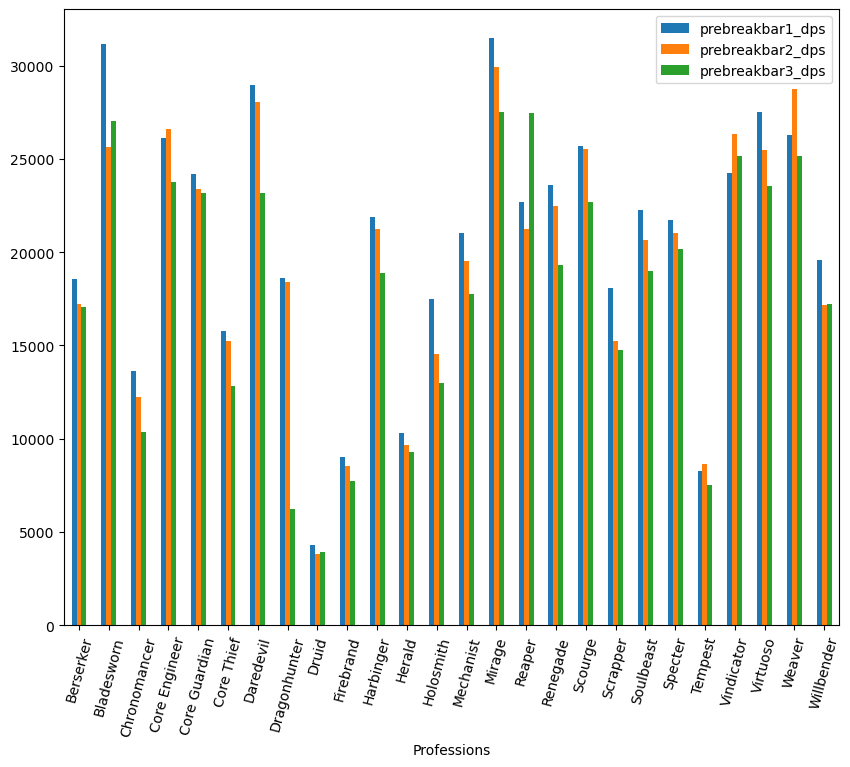
\includegraphics[width=0.9 \linewidth]{sh_dps_plot.png}
        \caption{Soulless Horror}
    \end{figure}

    \newpage

    \begin{figure}[h!]
        
        \centering
        
        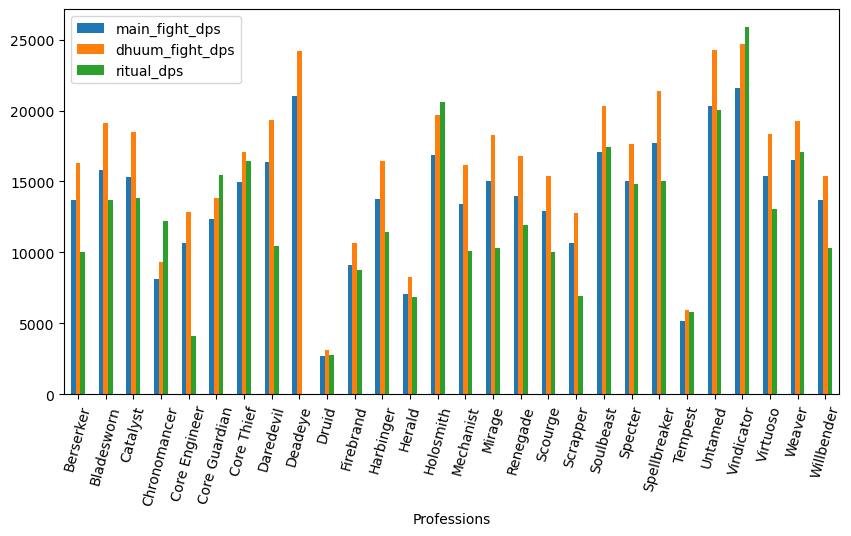
\includegraphics[width=1 \linewidth]{dhuum_dps_plot.png}
        \caption{Dhuum}
        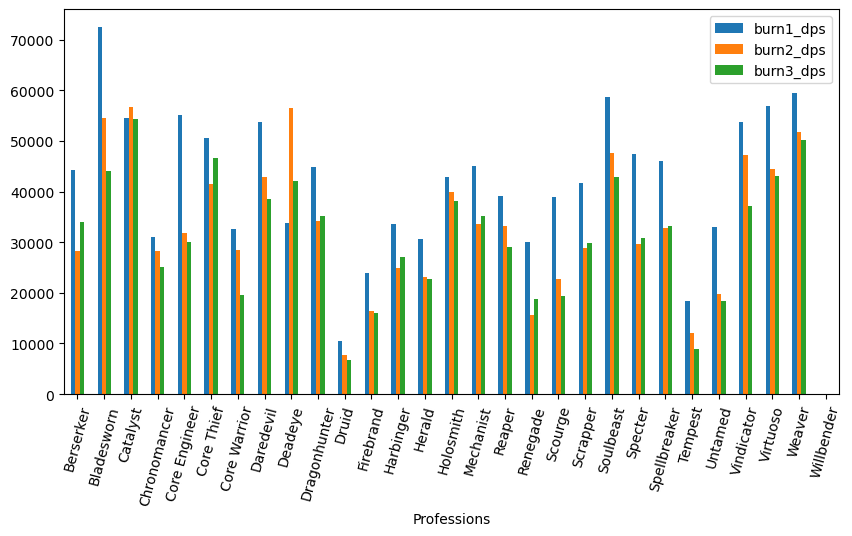
\includegraphics[width=1 \linewidth]{ca_dps_plot.png}
        \caption{Conjured Amalgamate}
    \end{figure}

    \newpage

    \begin{figure}[h!]
        
        \centering
        
        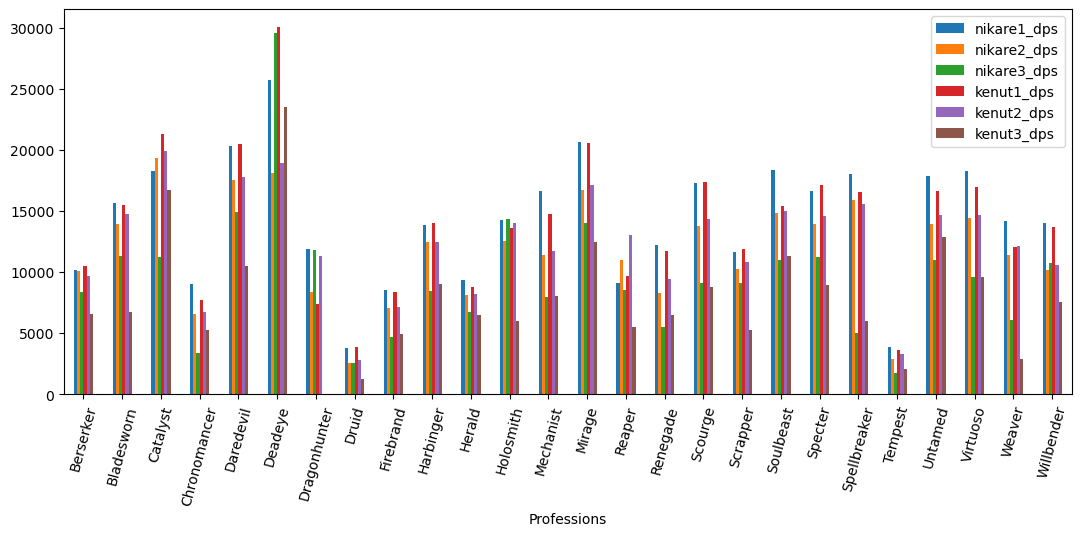
\includegraphics[width=1 \linewidth]{twins_dps_plot.png}
        \caption{Twin Largos}
        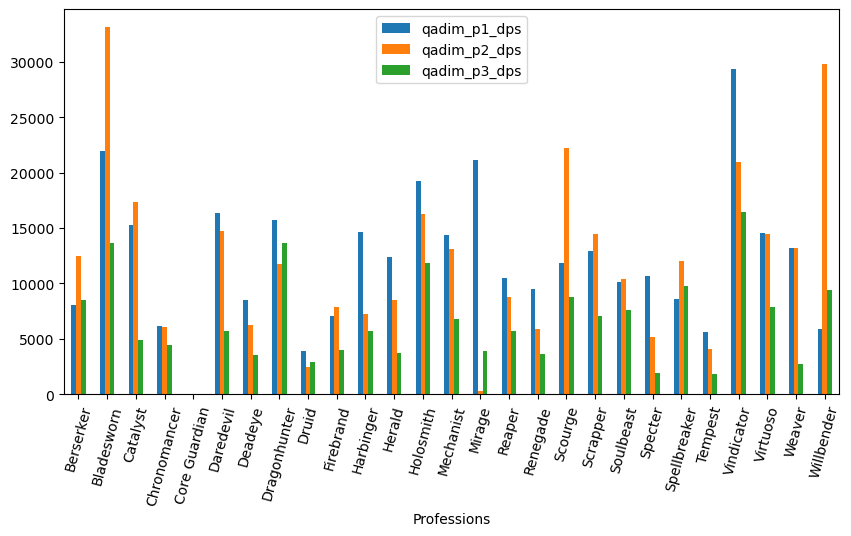
\includegraphics[width=1 \linewidth]{q1_dps_plot.png}
        \caption{Qadim}
    \end{figure}

    \newpage

    \begin{figure}[h!]
        
        \centering
        
        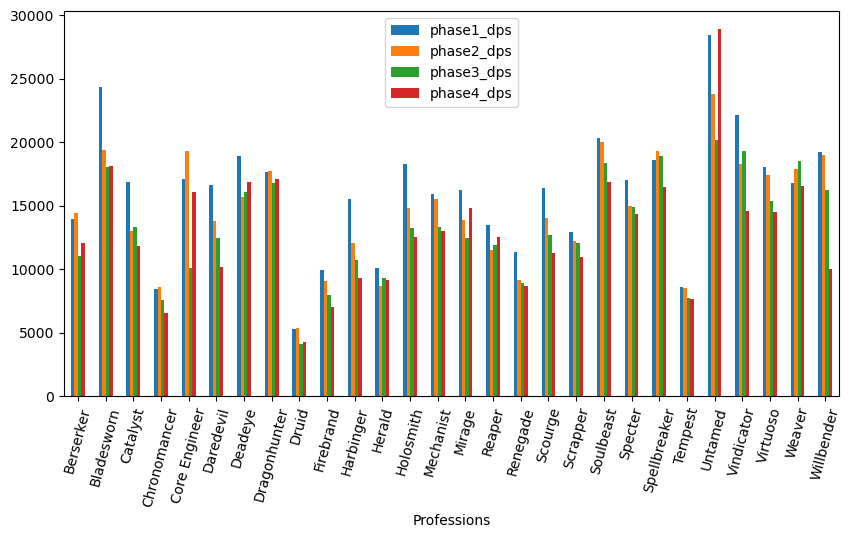
\includegraphics[width=1 \linewidth]{adina_dps_plot.png}
        \caption{Cardinal Adina}
        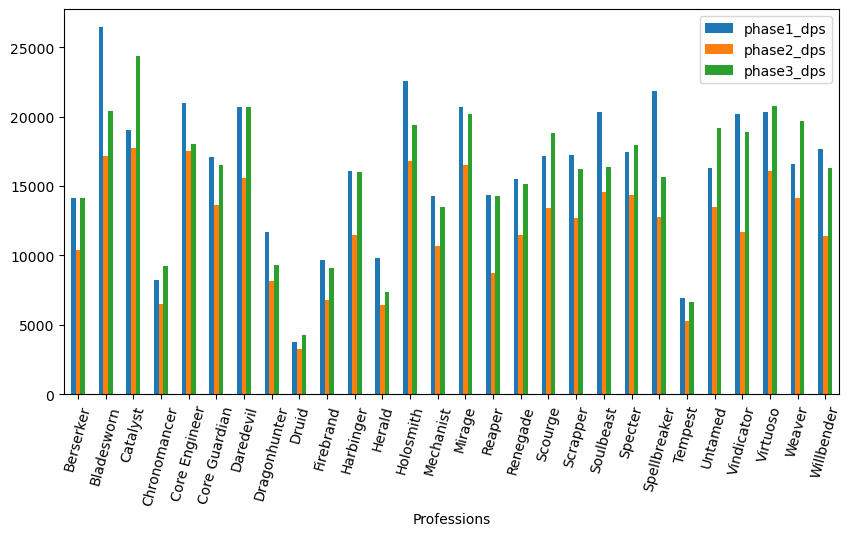
\includegraphics[width=1 \linewidth]{sabir_dps_plot.png}
        \caption{Cardinal Sabir}
    \end{figure}

    \newpage

    \begin{figure}[h!]
        
        \centering
        
        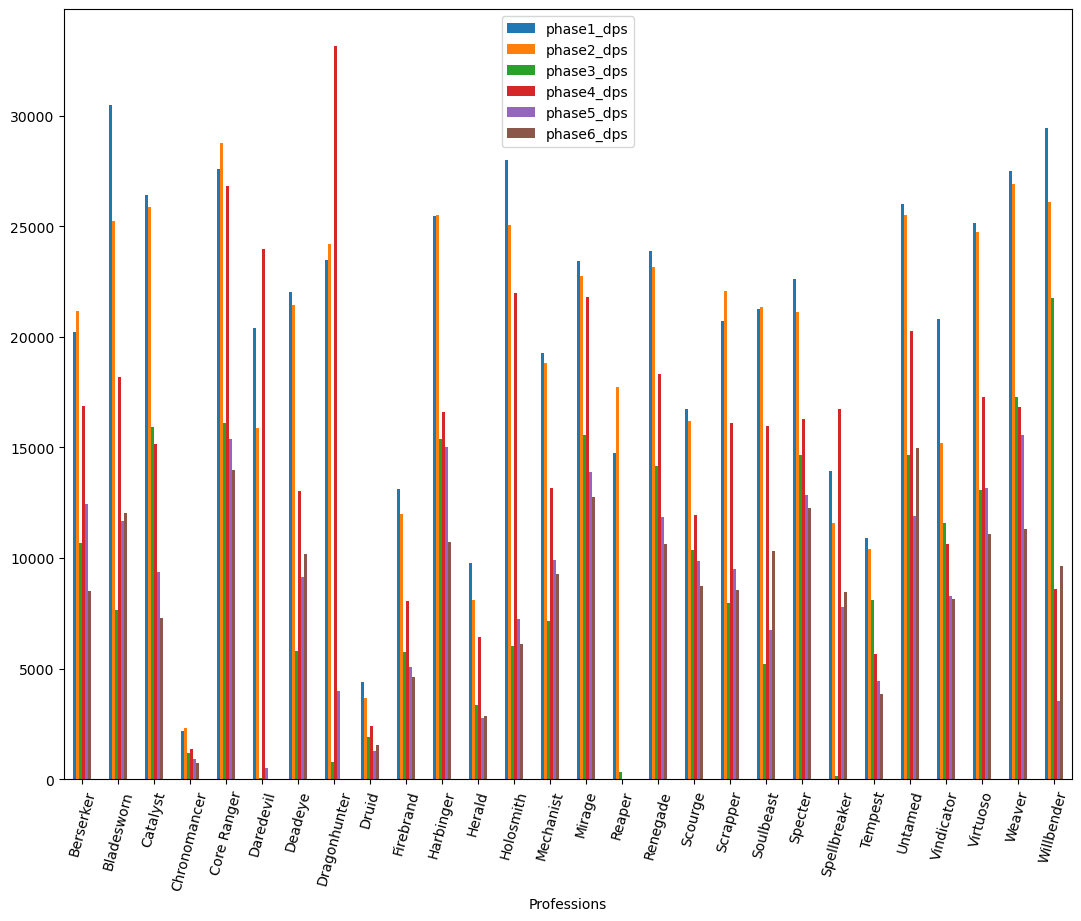
\includegraphics[width=1 \linewidth]{prlqadim_dps_plot.png}
        \caption{Qadim The Peerless}
    \end{figure}

    Twin Largos is a really special boss, because it actually contains two bosses in one fight, however, it is 
    separated between extremely clear phases that, in game, are specified by platforms. Each boss, Nikare and
    Kenut, have three platforms each, which define their phases quite well.\\

    As for Qadim The Peerless, classes like Scourges and Deadeyes are the ones playing a \textbf{Pylon} role
    and therefore, they are used almost a 90\% of the times.

    \newpage

    \subsection*{\normalsize 4.2.3 Analysis}

    \begin{wrapfigure}{r}{0.5\textwidth}
        \centering
        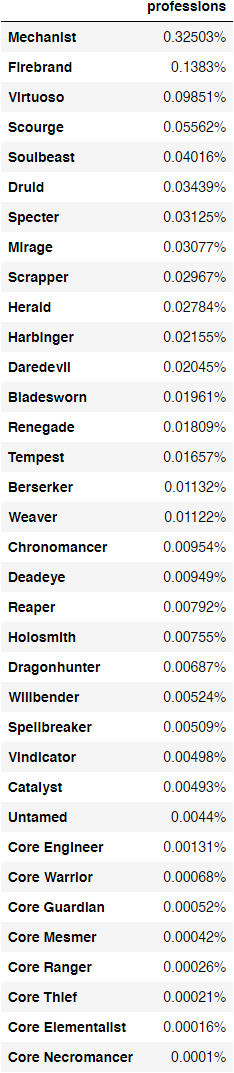
\includegraphics[scale=0.7]{class_percentage.png}
    \end{wrapfigure}

    After seeing all the previous graphs is quite obvious how some classes are used a lot more than others.
    This changes a lot as it is important to know that buffs and nerfs get done within the game after some 
    time, which in the end keeps the game balanced.\\

    \textbf{Important}: This whole project data analysis was made using the May to September 2022 status of
    the game, therefore, with future changes and also, more data, it's highly probable that results change.\\

    On this side figure, I wanted to show data in a more understandable format. All this results are based on
    a global table and, as it portrays, \textbf{Mechanist} and  \textbf{Firebrand} are the two classes with 
    higher usage on a global percentage. As I explained earlier, Mechanist is one of the most versatile classes
    the game ever had, and yes, other classes like Firebrand is also quite versatile. In terms of damage, this
    also varies from encounter to encounter but some professions still stand out more since they can have an 
    easier burst damage, which is essentially based on the class rotation.

    \newpage

    Rotations are the main damage source classes have, as guild web-pages like \textbf{Snowcrows} or \textbf{LuckyNoobs} made sure to
    optimize this so every player can make use of the class full potential by applying the correct ability order
    that creates several effects such as buffs, field effects and combos.\\

    \textbf{Extra}:\\
    To understand what \textbf{Snowcrows} and \textbf{LuckyNoobs} does, I will leave links to the pages but also, explain what they
    do and contribute to the Guild Wars 2 community. Since Fractals and Raids were release as new PvE modes, some 
    guilds and players tried to find ways to optimize how this stages could be cleared. This is how this guilds 
    were born, but they are not something new as they always existed on other games like World Of Warcraft for PvP.\\

    What they give to players are builds adapted to the current meta-game and they also revise them from time to time
    so all build are also up-to-date with new changes that Guild Wars team release into the game.

    \begin{itemize}
        \item SnowCrows \href{https://snowcrows.com/}{\textbf{here}}.
        \item LuckyNoobs \href{https://lucky-noobs.com/}{\textbf{here}}.
    \end{itemize}

    \bigskip

    \section*{\large Conclusion}
    This project helped me to understand a lot more how to work with data, from building my own algorithms and
    functions, to clean and extract important information from big chunks of data. I enjoyed this project a lot and I
    will keep enjoying it as this don't end just yet. I have in mind doing several optimizations to the code and also,
    building a Machine Learning algorithm to recommend new players the best class to use on each boss. I quite ambitious
    with what this project can lead to and I will expect developing more functionalities.

    \begin{figure}[b]
        \centering
        \begin{subfigure}[b]{0.15\linewidth}
            \href{https://github.com/icharo-tb}{
\includegraphics[width=\linewidth]{Images/GitHub-logo.png}}
        \end{subfigure}
        \begin{subfigure}[b]{0.15\linewidth}
            \href{https://www.linkedin.com/in/danielopezpajares/}{
\includegraphics[width=\linewidth]{Images/LinkedIn_Logo.png}}
        \end{subfigure}
        \begin{subfigure}[b]{0.15\linewidth}
            \href{https://gitlab.com/daniel.lopez.pajares.2021}{
\includegraphics[width=\linewidth]{Images/GitLab_logo.png}}
        \end{subfigure}
    \end{figure}
\end{document}